
\subsection{Expérience}
Un pendule électrostatique est constitué d'une petite boule de papier aluminium suspendu par un fil de coton à une potence ({\it fig. 1}).
 
Lorsqu'on frotte une règle en plastique avec un tissu en coton, des électrons sont arrachés du coton par la règle, la règle porte alors une charge négative, le tissu porte une charge positive.
% (le pendule n'est pas chargé mais la force de Coulomb crée une polarisation),

attire le pendule ({\it fig. 2}).


Lorsque le pendule touche le batonnet, un {\it transfert de charge} a lieu, le pendule se charge électriquement, et est alors repoussé ({\it fig. 3}).

\begin{center}
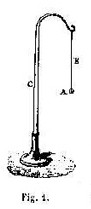
\includegraphics[scale=0.9]{./forces/Mascart01}
\hspace{0.3cm}
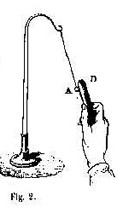
\includegraphics[scale=0.9]{./forces/Mascart02}
\hspace{0.3cm}
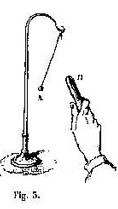
\includegraphics[scale=0.9]{./forces/Mascart03}
\end{center}

L'expérience du pendule électrostatique peut se modéliser par des {\it forces électrostatiques} s'exerçant entre des particules chargées.
%Ce modèle suppose une {\it action à distance}.

